\documentclass[border=4pt]{standalone}
\usepackage{amsmath,amssymb,tikz}
\usetikzlibrary{arrows.meta}
\begin{document}
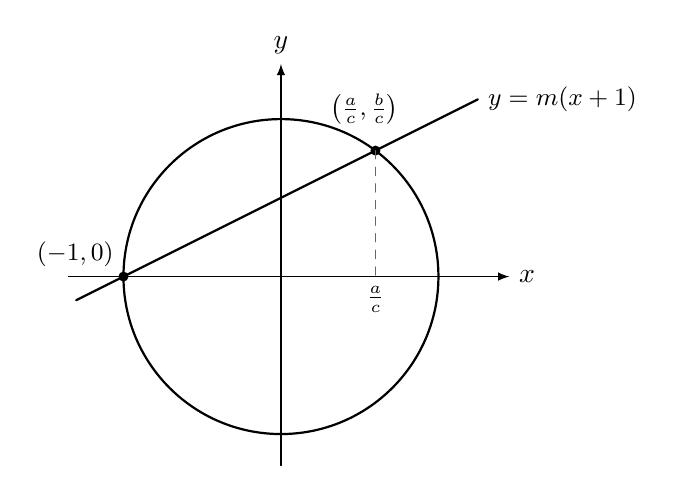
\begin{tikzpicture}[scale=2.0,>=latex,line cap=round]
  \draw[->] (-1.35,0) -- (1.45,0) node[right]{$x$};
  \draw[->] (0,-1.2) -- (0,1.35) node[above]{$y$};
  \draw[thick] (0,0) circle (1);
  % point (a/c,b/c) = (3/5,4/5), slope m = 1/2
  \draw[thick] (-1.3,-0.15) -- (1.25,1.125) node[right,font=\small]{$y = m(x+1)$};
  \fill (-1,0) circle (0.9pt) node[above left,font=\small]{$(-1,0)$};
  \fill (0.6,0.8) circle (0.9pt) node[above,font=\small,yshift=6pt,xshift=-4pt]{$\bigl(\tfrac ac,\tfrac bc\bigr)$};
  \draw[dashed,black!60] (0.6,0.8) -- (0.6,0);
  \node[below,font=\small] at (0.6,0) {$\tfrac ac$};
\end{tikzpicture}
\end{document}
